% Лабораторная работа по АСиСу № 7
% Михедов Константин Константинович

% Тип документа: статья, на бумаге А4
\documentclass[a4paper]{article}

% Подключение сторонних tex файлов 
\usepackage{import}


% Основные данные - ВУЗ, факультет, город...
\import{./../../stuff/tex}{config.tex}

% Подключение необходимых зависимостей
\import{./../../stuff/tex/settings}{packages.tex}
% Настройка подключенных пакетов
\import{./../../stuff/tex/settings}{preferences.tex}


% Шаблон титульной страницы 
\import{./../../stuff/tex/templates}{title.tex}
% Упрощенный блок "выполнил"
\import{./../../stuff/tex/templates}{sign1.tex}
% Макрос для содержания
\import{./../../stuff/tex/templates}{toc.tex}

% Определяем название документа
\title{
  Лабораторная работа №7 по курсу \\
  <<Компьютерный практикум <<Администрирование систем и сетей>>  
}
% Отключаем отображение правительства
\renewcommand{\government}{}
% Отключаем сокращенное нзавание университета
\renewcommand{\subuniversity}{}
% Указываем преподавателя
\renewcommand{\shortteachername}{Зудин Д.Е.}


% Путь до внешних изображений
\graphicspath{ {./figures/}}


% Основной текст работы
\begin{document}
  \templatedtitlepage
  
  \toc
  \section{Ход работы}

  \subsection{Задание}

  Выполнен 9 вариант, для которого указан сетевой адрес 10.15.10.0 и следующая
  топология сети:

  \begin{figure}[H]
    \centering
    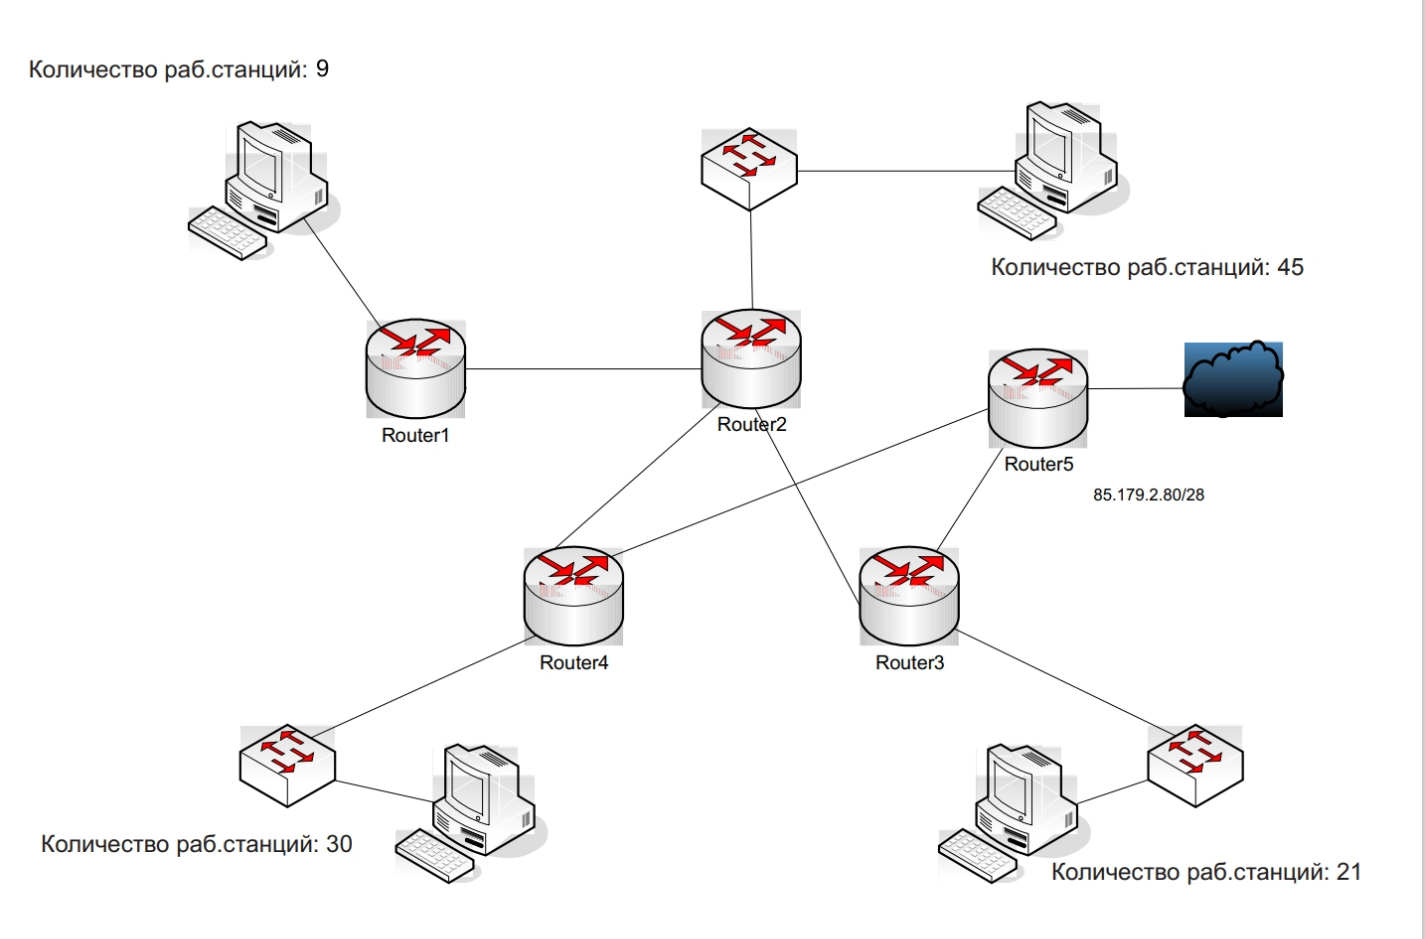
\includegraphics[width=0.85\textwidth]{07}
    \caption{Топология сети для 9 варианта}
    \label{img:topology}
  \end{figure}

  \newpage
  \subsection{Формирование подсетей}

  По данной топологии можно выделить несколько различных подсетей, выпишем их в 
  таблицу с указанием участников и присвоением имен:
  \begin{table}[H]
    \centering
    \begin{tabular}{| c | c | c | c |}
      \hline
      Имя & Участники & Кол-во узлов & Особенности \\
      \hline
      R2-45W & Router2 и 45 раб. станций & 46 & - \\
      \hline
      R4-30W & Router4 и 30 раб. станций & 31 & - \\
      \hline
      R3-21W & Router3 и 21 раб. станция & 22 & - \\
      \hline
      R1-9W & Router1 и 9 раб. станций & 10 & Нет свитча$\left(\right.$ \\
      \hline
      R1-R2 & Router1 и Router2 & 2 & Всего 2 участника \\
      \hline
      R2-R3 & Router2 и Router3 & 2 & Всего 2 участника \\
      \hline
      R2-R4 & Router2 и Router4 & 2 & Всего 2 участника \\
      \hline
      R3-R5 & Router3 и Router5 & 2 & Всего 2 участника \\
      \hline
      R4-R5 & Router4 и Router5 & 2 & Всего 2 участника \\
      \hline
      R5-Ex & Router5 & 1 & Выход в стороннюю сеть \\      
      \hline
    \end{tabular}
    \caption{Выделенные подсети}
  \end{table}

  Для каждой выделенной подсети необходимо определить ее собственный адрес, а также
  маску подсети. Сделаем это для каждой подсети в порядке уменьшения количества узлов:
  \begin{enumerate}
    \item {
      \textbf{Подсеть R2-45W}

      В данной подсети содержиться 46 различных узлов, также требуется 2 дополнительных
      адреса - один для сети в целом, один для широковещательной отправки пакетов,
      итого подсеть должна включать 48 \textit{IP} адресов. Наименьшее ближайшее к этому
      количеству число, являющееся степенью двойки, 64, то есть на всю подсеть будет
      выделено 64 адреса, что соответсвует маске 255.255.255.192.

      Назначим данной подсети адрес. Так как еще ни один адрес из исходной сети не
      распределен, используем первый возможный - 10.15.10.0.

      С учетом маски, первый доступный \textit{IP} адрес в этой сети 10.15.10.1,
      последний - 10.15.10.62 и широковещательный - 10.15.10.63.
    }
    \item {
      \textbf{R4-30W}

      Данная подсеть содержит 31 узла, также требует 2 дополнительных адреса,
      итого получается, что она должна включать минимум 33 адреса. Ближайшая
      большая степень двойки снова 64, то есть этой подсети также выдадим маску
      255.255.255.192.

      Так как адреса с 10.15.10.0 по 10.15.10.63 уже заняты, то адресом
      данной подсети назначим первый свободный - 10.15.10.64.

      Исходя из маски и адреса сети выделим первый доступный \textit{IP}
      10.15.10.65, последний - 10.15.10.126 и широковещательный - 10.15.10.127.
    }
    \item {
      \textbf{R3-21W}

      Подсеть содержит 22 узла, требует 2 дополнительных адреса, итого необходимо 24 адреса.
      Для такого размера подходит маска 255.255.255.224 (32 адреса всего).

      Первый свободный адрес родительской сети - 10.15.10.128. Его же назначим адресом
      данной подсети.

      С учетом маски, первый доступный \textit{IP} адрес - 10.15.10.129, последний - 10.15.10.158,
      широковещательный - 10.15.10.159.
    }
    \item {
      \textbf{R1-9W}

      Подсеть на 10 узлов, требуется два дополнительных адреса, итого вся подсеть
      должна включать минимум 12 адресов. Ближайщая степень двойки - 16, что соответсвует
      маске 255.255.255.240.

      В качестве адреса сети назначим адрес 10.15.10.160, тогда первый доступный \textit{IP} адрес - 10.15.10.161,
      последний - 10.15.10.174, широковещательный - 10.15.10.175.
    }
    \item {
      \textbf{R1-R2}

      Подсеть всего на 2 участника (точка-точка), по умолчанию выдаем ей маску 255.255.255.252.
      Назначим ей адрес - 10.15.10.176, тогда первый доступный \textit{IP} адрес - 10.15.10.177, последний -
      10.15.10.178, широковещательный - 10.15.10.179.
    }
    \item {
      \textbf{R2-R3}

      Подсеть всего на 2 участника (точка-точка), по умолчанию выдаем ей маску 255.255.255.252.
      Назначим ей адрес - 10.15.10.180, тогда первый доступный \textit{IP} адрес - 10.15.10.181, последний -
      10.15.10.182, широковещательный - 10.15.10.183.
    }
    \item {
      \textbf{R2-R4}

      Подсеть всего на 2 участника (точка-точка), по умолчанию выдаем ей маску 255.255.255.252.
      Назначим ей адрес - 10.15.10.184, тогда первый доступный \textit{IP} адрес - 10.15.10.185, последний -
      10.15.10.186, широковещательный - 10.15.10.187.
    }
    \item {
      \textbf{R3-R5}

      Подсеть всего на 2 участника (точка-точка), по умолчанию выдаем ей маску 255.255.255.252.
      Назначим ей адрес - 10.15.10.188, тогда первый доступный \textit{IP} адрес - 10.15.10.189, последний -
      10.15.10.190, широковещательный - 10.15.10.191.
    }
    \item {
      \textbf{R4-R5}

      Подсеть всего на 2 участника (точка-точка), по умолчанию выдаем ей маску 255.255.255.252.
      Назначим ей адрес - 10.15.10.192, тогда первый доступный \textit{IP} адрес - 10.15.10.193, последний -
      10.15.10.194, широковещательный - 10.15.10.195.
    }
    \item {
      \textbf{R5-Ex}

      Данная подсеть уже имеет назначенный адрес - 85.179.2.80/28. По нему видно,
      что маска данной подсети - 255.255.255.240, сама подсеть может включать 16 различных
      адресов (14 узлов) и имеет широковещательный адрес 85.179.2.95.

      Для Router5 в этой подсети можно выделить первый достпуный адрес - 85.179.2.81.
    }
  \end{enumerate}

  Сведем результаты расчетов в таблицу:
  \begin{table}[H]
    \centering
    \begin{tabular}{| c | c | c | c |}
      \hline
      Подсеть & Адрес сети & Маска сети & Широковещательный \\
      \hline
      R2-45W & 10.15.10.0 & 255.255.255.192 & 10.15.10.63 \\
      \hline
      R4-30W & 10.15.10.64 & 255.255.255.192 & 10.15.10.127 \\
      \hline
      R3-21W & 10.15.10.128 & 255.255.255.224 & 10.15.10.159 \\
      \hline
      R1-9W & 10.15.10.160 & 255.255.255.240 & 10.15.10.175 \\
      \hline
      R1-R2 & 10.15.10.176 & 255.255.255.252 & 10.15.10.179 \\
      \hline
      R2-R3 & 10.15.10.180 & 255.255.255.252 & 10.15.10.183 \\
      \hline
      R2-R4 & 10.15.10.184 & 255.255.255.252 & 10.15.10.187 \\
      \hline
      R3-R5 & 10.15.10.188 & 255.255.255.252 & 10.15.10.191 \\
      \hline
      R4-R5 & 10.15.10.192 & 255.255.255.252 & 10.15.10.195 \\
      \hline
      R5-Ex & 85.179.2.80 & 255.255.255.240 & 85.179.2.95 \\
      \hline
    \end{tabular}
    \caption{Итоговое распределение}
  \end{table}

  \subsection{Итоговая сеть}

  Все выделенные подсети заняли \textit{IP} адреса в диапазоне 10.15.10.0 - 10.15.10.195,
  то есть 195 штук. Для того, чтобы вместить столько узлов, потребуется сеть на 256 адресов (
  ближайшая большая степень двойки), что соответсвует маске 255.255.255.0.

  Тогда минимальная возможная сеть, включающая в себя все выделенные подсети, была бы
  с адресом 10.15.10.0/24.

  \newpage
  \section{Вывод}

  В ходе данной Лабораторной работы мной были получены навыки выделения подсетей, расчета
  масок и выведения широковещательного и сетевого адресов с ее помощью.

\end{document}
